\section{Variance propagation}

\begin{figure*}[t]
    \centering
    \begin{subfigure}{.5\textwidth}
        \centering
        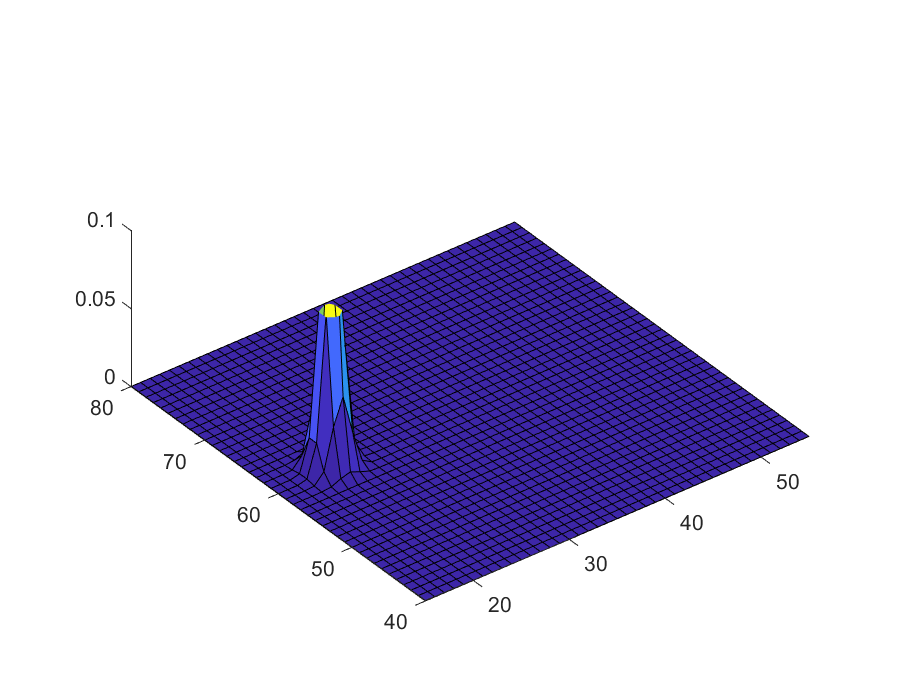
\includegraphics[width=\linewidth]{Figures/PDF_t0}
        \caption{t=0s}
        \label{fig:PDF_initial}
    \end{subfigure}%
    \begin{subfigure}{0.5\textwidth}
        \centering
        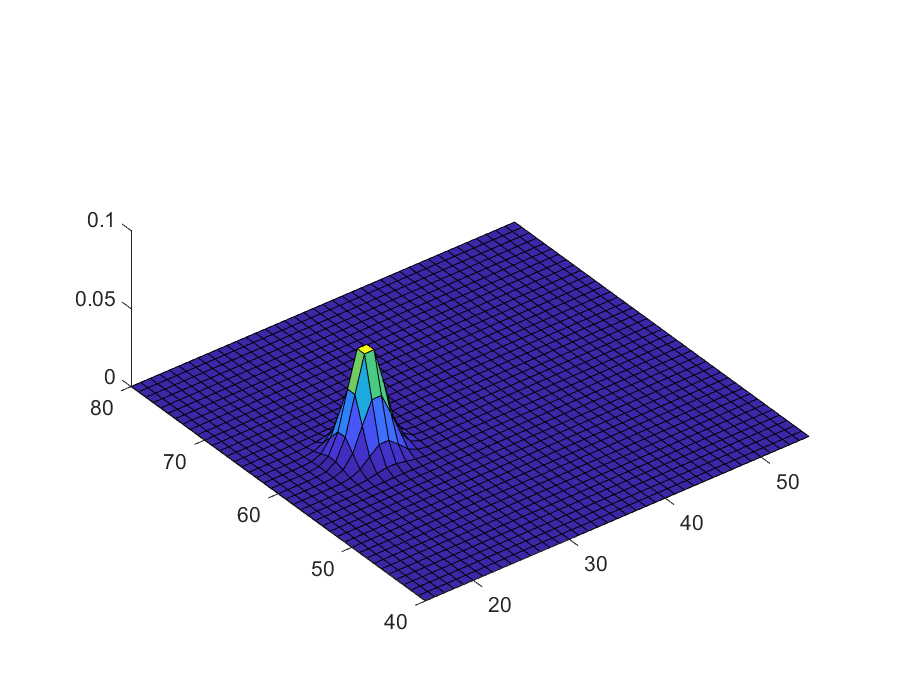
\includegraphics[width = \linewidth]{Figures/PDF_t5}
        \caption{t=5s}
        \label{fig:PDF_t5}
    \end{subfigure} \\
    \begin{subfigure}{.5\textwidth}
        \centering
    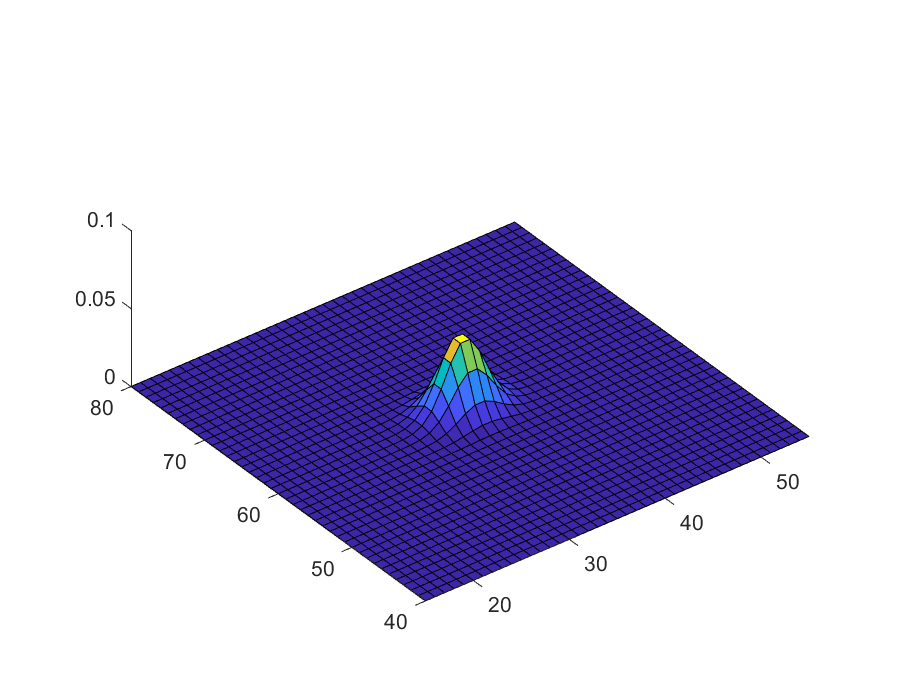
\includegraphics[width=\linewidth]{Figures/PDF_t15}
    \caption{t=15s}
    \label{fig:PDF_t15}
    \end{subfigure}%
    \begin{subfigure}{0.5\textwidth}
        \centering
    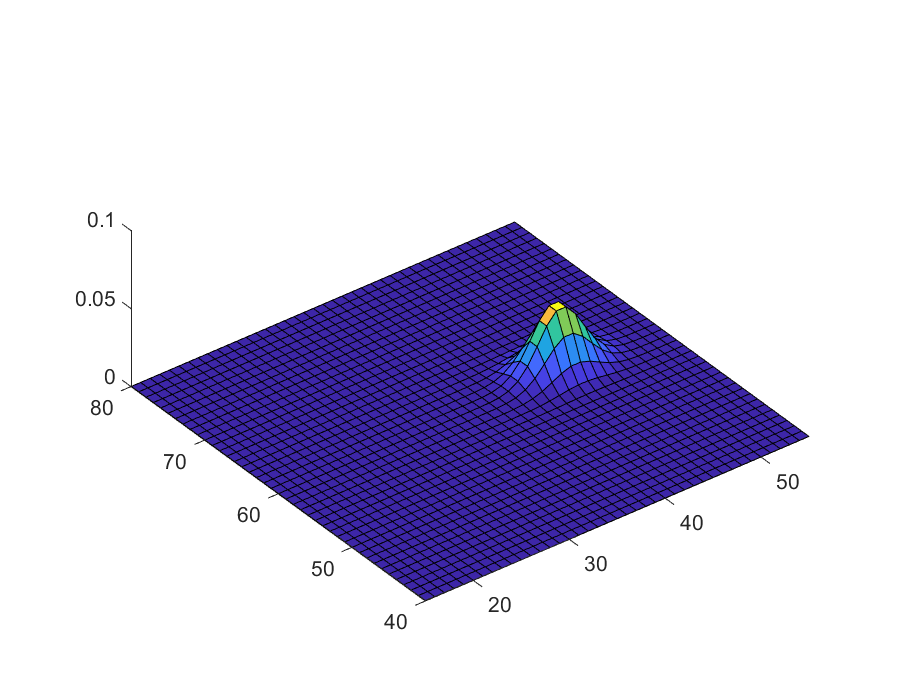
\includegraphics[width=\linewidth]{Figures/PDF_t20}
    \caption{t=20s}
    \label{fig:PDF_t20}
    \end{subfigure} 
    \caption{The probability density functions over the drone position at different time-steps in the simulation done by the MPC.}
    \label{fig:PDF_development}
\end{figure*}

\subsection{Varaince formulation}

To be able to propagate the variance through the system a linear system is required. The state space is linear, but the LOS guidance law is nonlinear due to the normalization of the $\chi^{NED}_{los,ca}$ vector in equation \eqref{V_ref,ca}. Nonlinearities will make a Gaussian curve loose its form making it difficult to propagate the system further.The system is linearized to compensate for this problem.

First the guidance law is re-written.

\begin{align}
    \chi^{NED}_{los,ca} & = R^{NED}_{los}  R_{ca} \left(  \begin{bmatrix}\Delta \\ 0 \\ 0\end{bmatrix} - \begin{bmatrix} 0 & 0 & 0 \\ 0 & 1 & 0 \\ 0 & 0 & 1 \end{bmatrix} R^{los}_{NED} (\begin{bmatrix} \mathbf{I} & \mathbf{0} \end{bmatrix} \hat{x} - WP_1) \right) \\
    & = E - F \hat{x}_p \\
     & = E - F x_p - F v_p \\
    E & = R^{NED}_{los}  R_{ca} \left(  \begin{bmatrix}\Delta \\ 0 \\ 0\end{bmatrix} + \begin{bmatrix} 0 & 0 & 0 \\ 0 & 1 & 0 \\ 0 & 0 & 1 \end{bmatrix} R^{los}_{NED} WP_1 \right) \\
    F & = R^{NED}_{los}  R_{ca}  \begin{bmatrix} 0 & 0 & 0 \\ 0 & 1 & 0 \\ 0 & 0 & 1 \end{bmatrix} R^{los}_{NED}\\
    x_p & = \begin{bmatrix}\mathbf{I}  &\mathbf{0}\end{bmatrix} x, \quad 
    \hat{x}_p  = \begin{bmatrix}\mathbf{I}& \mathbf{0}\end{bmatrix} \hat{x}, \quad
    v_p  = \begin{bmatrix}\mathbf{I}& \mathbf{0}\end{bmatrix} v 
\end{align}

Both x and v are stocastic variabels.$x$ contains the uncertainty in the state, $v$ describes the added uncertainty due to measurement errors. 

\begin{align}
        V_{ref,ca} & = v_0 \frac{\chi^{NED}_{los,ca} }{|| \chi^{NED}_{los,ca} ||} \\
        V_{ref,ca} & = v_0 \frac{E - F x_p - F v_p }{|| E - F x_p - F v_p ||}
\end{align}

This equation is linearized around the current expected $x$ value, $x=x_0$, and the expected value of the noise $v=v_0=0$. The expected $x$ value is calculated by the state space equation. The linearization is done in appendix A. This results in the following linearized equation

\begin{align}
        \bar{V}_{ref,ca}  ={}& v_0 (\bar{E} - \bar{F} x -\bar{F} v) \\
        \bar{E} ={}&  G + H \begin{bmatrix}\mathbf{I}  &\mathbf{0}\end{bmatrix} x_0 \\
        \bar{F} ={}& H \begin{bmatrix}\mathbf{I}  &\mathbf{0}\end{bmatrix} \\
        G ={}& \frac{E - F \begin{bmatrix}\mathbf{I}  &\mathbf{0}\end{bmatrix} x_0}{||E - F \begin{bmatrix}\mathbf{I}  &\mathbf{0}\end{bmatrix} x_0||} \\
        H ={}& \frac{F}{||E - F \begin{bmatrix}\mathbf{I}  &\mathbf{0}\end{bmatrix} x_0||}\\
                &-\left(\frac{(E - F \begin{bmatrix}\mathbf{I}  &\mathbf{0}\end{bmatrix} x_0)(E - F \begin{bmatrix}\mathbf{I}  &\mathbf{0}\end{bmatrix} x_0)^\top F}{||E - F \begin{bmatrix}\mathbf{I}  &\mathbf{0}\end{bmatrix} x_0||^3}\right)
\end{align}

Inserting the linearized velocity reference vector into the state space equation

\begin{align}
 x[k+1] & = A_{cl} x[k] + B_{cl} \bar{V}_{ref}[k] - \Gamma_{cl} v[k] +w_d[k] \\
 \bar{V}_{ref} & = v_0 (\bar{E} - \bar{F} x -\bar{F} v)
\end{align}

Resulting in
\begin{align}
 & x[k+1]   = A_{los} x[k] + \Gamma_{los} v[k] + w_d[k] + C_{los} \\ \label{linearized_los_eq}
 & A_{los}  = A_{cl} - B_{cl} v_0 \bar{F}, \quad \Gamma_{los} =  -\Gamma_{cl} - B_{cl} v_0 \bar{F})\\ & C_{los} = B_{cl} v_0 \bar{E}
\end{align}

We now have a linear state space formulation. With the asumption that $v[k]$ and $w[k]$ are white noise processes, all the terms in \eqref{linearized_los_eq} become uncorrelated and the covariance matrix of $x[k+1]$ can simply be calculated as

\begin{align}
    \textnormal{var}(x[k+1]) &= A_{los} \textnormal{var}(x[k]) A_{los}^\top + \Gamma \textnormal{var}(v[k]) \Gamma^\top + \textnormal{var}(w_d[k])  \\
    \textnormal{var}(x[k+1]) &= A_{los} \textnormal{var}(x[k]) A_{los}^\top + \Gamma R_d \Gamma^\top + Q_d
\end{align}

The initial variance is equal the position estimate variance, $R_d$. 
\begin{align}
    \textnormal{var}(x[0]) &= R_d
\end{align}

\subsection{Results}

%\begin{figure}[t]
    %\centering
    %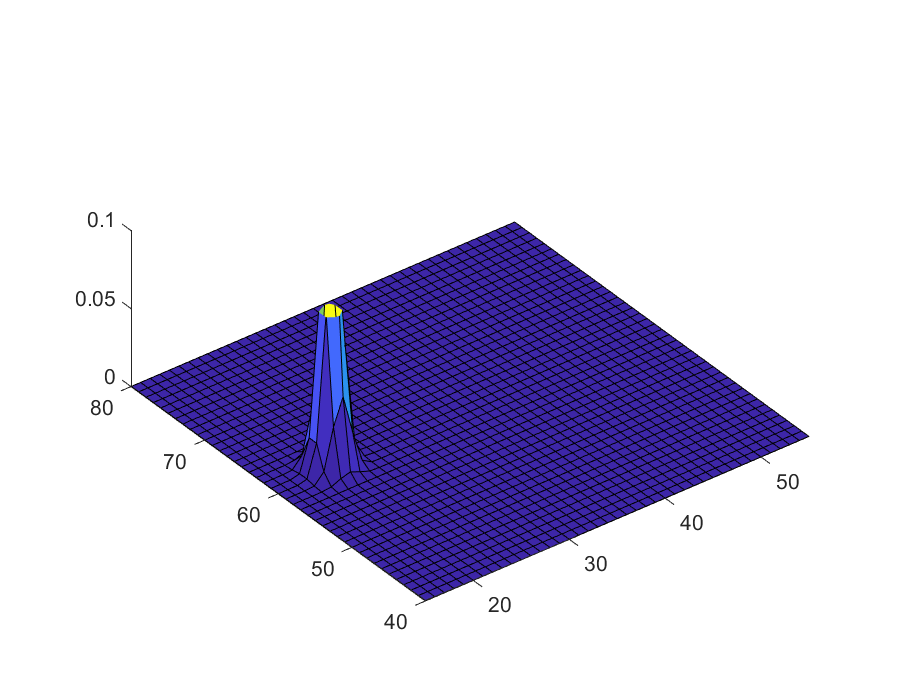
\includegraphics[width=\linewidth]{Figures/PDF_t0}
    %\caption{The initial probability density function of the drone position}
    %\label{fig:PDF_initial}
%\end{figure}

%\begin{figure}[t]
    %\centering
    %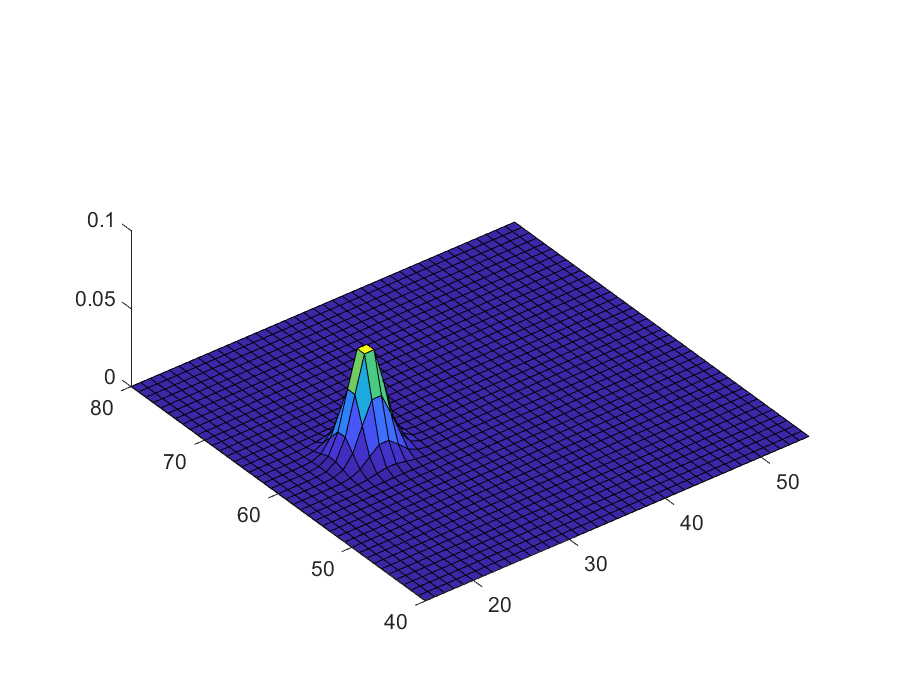
\includegraphics[width = \linewidth]{Figures/PDF_t5}
    %\caption{The probability density function of the drone position at t=5s}
    %\label{fig:PDF_t5}
%\end{figure}

%\begin{figure}[t]
    %\centering
    %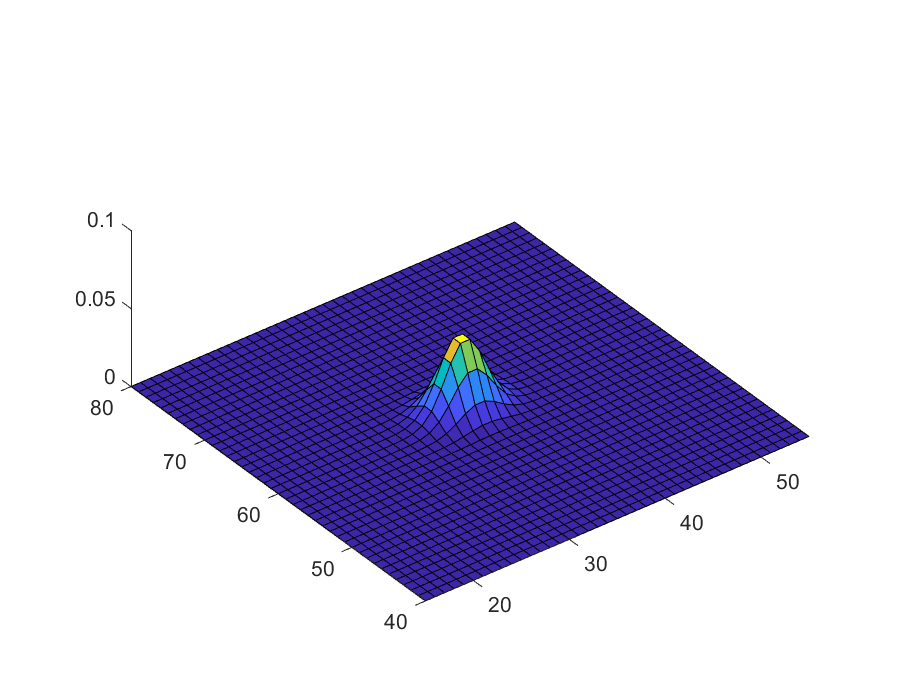
\includegraphics[width=\linewidth]{Figures/PDF_t15}
    %\caption{The probability density function of the drone position at t=15s}
    %\label{fig:PDF_t15}
%\end{figure}

%\begin{figure}[t]
    %\centering
    %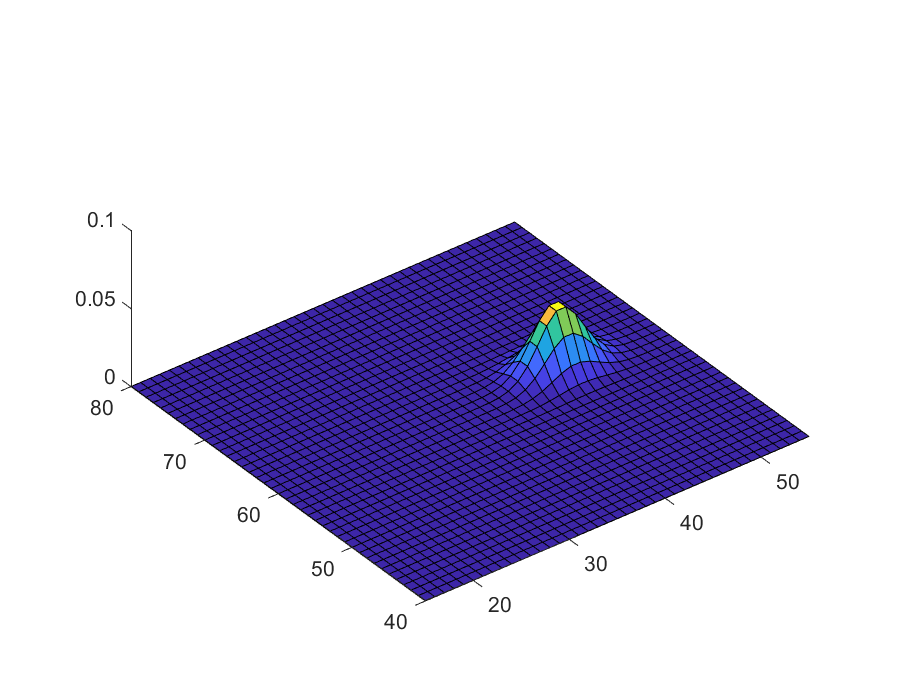
\includegraphics[width=\linewidth]{Figures/PDF_t20}
    %\caption{The probability density function of the drone position at t=20s}
    %\label{fig:PDF_t20}
%\end{figure}

The uncertainty in position will start low as and then gradually increase as seen in figure \ref{fig:PDF_development}. Its interesting to note that the probability density function becomes elongated over time, the uncertainty is larger in the along path direction than in the across path direction. This is a direct consequence of LOS guidance being asymptotically stable in across path direction, but only marginally stable in the along path direction, since the LOS guidance law does not try to counteract along path errors.